\newcommand{\MG}{\textsc{madgraph5}\xspace}
\newcommand{\MCNLO}{\textsc{mc@nlo}\xspace}
\newcommand{\aMCNLO}{\textsc{amc@nlo}\xspace}
\newcommand{\madgraph}{\textsc{madgraph5\_amc@nlo}\xspace}
\newcommand{\sherpa}{\textsc{sherpa}\xspace}
\newcommand{\OPENLOOPS}{\textsc{openloops}\xspace}
\newcommand{\powheg}{\textsc{powheg}\xspace}
\newcommand{\powhegbox}{\textsc{powheg-Box}\xspace}
\newcommand{\pythia}{\textsc{pythia}\xspace}
\newcommand{\herwig}{\textsc{herwig}\xspace}
\newcommand{\FxFx}{\textsc{FxFx}\xspace}
\newcommand{\MEPSNLO}{\textsc{MePs@NLO}\xspace}
\newcommand{\UNLOPS}{\textsc{UNLOPS}\xspace}
\newcommand{\MiNLO}{\textsc{MiNLO}\xspace}
\newcommand{\MADSPIN}{\textsc{MadSpin}\xspace}
\newcommand{\geant}{\textsc{Geant4}\xspace}
\newcommand{\afast}{\textsc{AtlFast-II}\xspace}
\newcommand{\evtgen}{\textsc{EvtGen}\xspace}
\newcommand{\toppp}{\textsc{Top}$_{++}$\xspace}
\newcommand{\COMIX}{\textsc{Comix}\xspace}
\newcommand{\PDFLHC}{\textsc{PDF4LHC}\xspace}
\newcommand{\tth}{\ensuremath{t\bar{t}H}\xspace}
\newcommand{\ctdiez}{\textsc{CT10NLO}\xspace}

\section{Proton-Proton event simulation}
\label{sec:event}

In this section, the modeling of proton-proton collisions occurring at the LHC is presented, which comprises several stages~\cite{BUCKLEY2011145}.
Firstly, the production cross-section for the hard scattering introduced previously in Section~\ref{subsec:proton} is calculated, describing the interactions between the partons that compose the incoming protons.
This is followed by parton showering, where gluon emissions and parton splitting are simulated. The next step involves hadronization, where resulting partons combine to form color-neutral hadrons, which subsequently decay along with other unstable particles. Additionally, the modeling of pile-up and underlying events, originating from multiple simultaneous proton interactions beyond the primary scattering within the same bunch crossing, is included.
Finally, events undergo detector simulation, digitization, and the same reconstruction algorithms used for real data, ensuring a realistic representation of experimental conditions.
Figure~\ref{fig:pdfs} illustrates the aforementioned steps involved in simulating a proton-proton collision.
\begin{figure}[htbp]
    \centering
    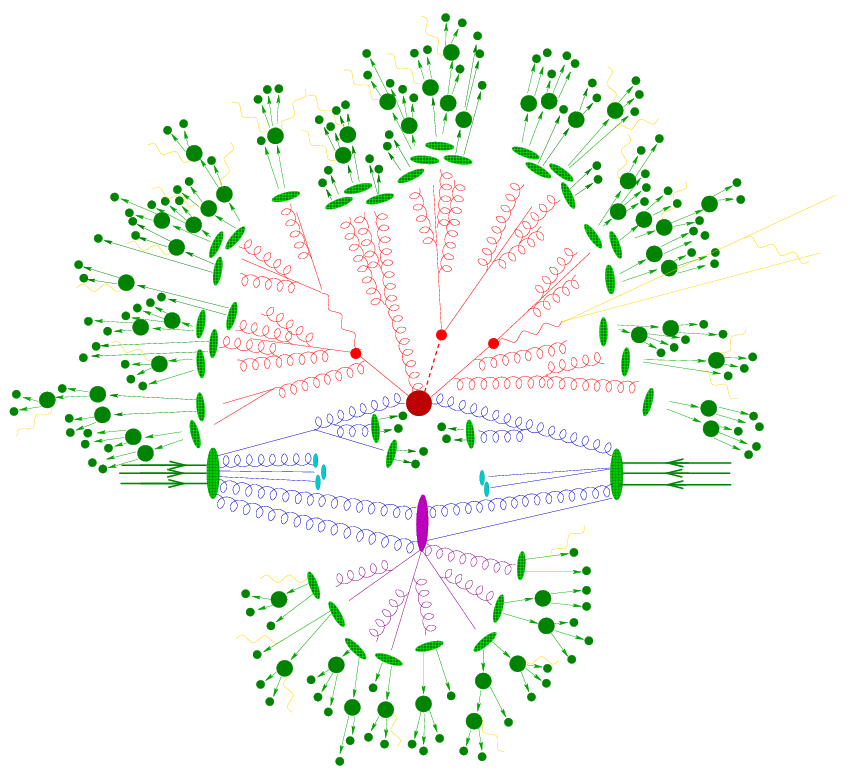
\includegraphics[width=0.9\textwidth]{images/atlas_pp_sim.png}
    \caption{Representation of components relevant for simulating a proton-proton collision event containing all the factorised stages, excluding pile-up~\cite{Gleisberg_2009}. The central red blob represents the hard-scattering of incident protons,
    while in blue it shows the initial partons that contributed. Additional hard QCD radiation, outgoing partons and their decays are also represented in red. In light green ellipses it is represented the hadronization of final state partons, while the decay
    of the resulting hadrons is represented by dark green regions with arrows. The partons that did not participate in the primary interaction conform the underlying event, in purple. In yellow one can find the photon radiation, that can occur at any stage.}
    \label{fig:pdfs}
  \end{figure}

\subsection{Matrix element and parton showers}
\label{subsec:parton_shower}
Given the large momentum transfer involved in the hard scattering processes at the LHC, the partonic cross-sections can be computed using perturbative QCD. In this framework, partons may radiate additional gluons and split into quarks, which in turn can emit yet more radiation both in the initial and final states. Computing the full cross-section ($\hat{\sigma})$ therefore requires summing over all possible quark/gluon emissions, which can be expressed as the perturbative expansion:
\begin{equation}
\hat{\sigma}(ij\rightarrow X) = \sum_{n=0}^{\infty}\int d\Phi_{X+n}\abs{\sum_{k=0}^{\infty}|\mathcal{M}_{X+n}^{^{(k)}}}|^2,
\end{equation}
being $\mathcal{M}_{X+n}^{^{(k)}}$ the matrix element for the process $ij \rightarrow X + n$, with $n$ the number of additional partons produced in the final state, $k$ the number of included virtual loops, and $d\Phi_{X+n}$ the phase space element for this process.
The calculation at LO only includes tree level matrix elements so it would correspond to $n=0$ and $k=0$. If the process involves the production of $N$ partons in the final state, then in this case the LO calculation for the process $ij \rightarrow X+N$ will involve $n=N$ and $k=0$.
In the same way, a matrix element calculation with $k + n = m$ is referred to as a calculation at $\text{N}^{\text{m}}$LO, for $ij \rightarrow X$.

This is how the cross-sections are calculated precisely for such scattering processes. However, when too many partons appear in the final state the computation becomes prohibitively expensive, so the matrix elements are evaluated only up to a certain order in the strong coupling constant
 $\alpha_{s}$ (see Eq.~\ref{running}), and the remainder is approximated via the parton-showering algorithm, where the showering is simulated using approximate matrix elements~\cite{FOX1980285}.

%%Because parton emissions span a wide range of energy scales, the phase space accessible to a parton-shower algorithm inevitably overlaps with that already covered by higher-multiplicity matrix elements. If left untreated, this overlap would double-count contributions and decrease the accuracy of cross-section and jet-multiplicity predictions, especially when an energetic, wide-angle emission converts an n-jet configuration into an (n + 1)-jet one.
%%Matching and merging prescriptions resolve the overlap by defining, event-by-event, which emissions originate from the fixed-order calculation and which from the shower. Slicing techniques introduce a matching scale: high-pT, large-angle partons are described by multi-leg matrix elements, while softer or more collinear radiation is delegated to the shower, preserving leading-logarithmic accuracy without duplication. Widely used implementations include 
%%the geometrical MLM~\cite{MANGANO2002343} algorithm and the CKKW~\cite{Catani_2001} schemes, which re-weight matrix elements and constrain subsequent showering; their next-to-leading-order extension is known as FxFx~\cite{Frederix_2012}. By combining samples of increasing jet multiplicity under these rules, one obtains inclusive event samples that smoothly interpolate between the hard and soft regimes.
Matching and merging schemes prevent double counting between high-multiplicity matrix elements and the parton shower by assigning emissions above a chosen matching scale to fixed-order calculations and relegating softer or collinear radiation to the shower. Widely used approaches, such as the MLM algorithm~\cite{MANGANO2002343} and CKKW schemes~\cite{Catani_2001} with their NLO extension FxFx~\cite{Frederix_2012}, combine tree-level multileg samples
of increasing jet multiplicity with parton showers to produce inclusive event samples that smoothly interpolate between hard, wide-angle emissions and soft, collinear radiation.

\subsection*{Hadronization}
\label{subsec:Hadronization}

Below the perturbative cutoff of order 1 GeV, parton showering hands off to non-perturbative hadronization, during which coloured partons (each carrying definite momentum, flavour and colour) are clustered into colour-neutral hadrons. Phenomenological models such as the Lund string model or the cluster model take over here.

In the Lund string model~\cite{ANDERSSON198331} the colour field between a quark and an antiquark is treated as a relativistic string whose potential energy rises with separation; when that energy exceeds the mass of a new $q\bar{q}$ pair the string breaks, repeatedly creating additional pairs until all energy is exhausted, with hadron momenta drawn from an empirical fragmentation function. 
The cluster model~\cite{Winter_2004} instead splits each final-state gluon into a $q\bar{q}$ pair and groups them into colour-singlet clusters; those clusters then undergo a cascade of decays, or directly fragment, until only stable hadrons remain.

\subsection*{Pile-up and underlying event}
\label{subsec:Pile}

All activity and interactions occurring in a proton-proton collision beyond the primary hard scattering must also be modelled; these are referred to as the underlying event and pile-up backgrounds, as discussed in Section~\ref{sec:LHC}. 
In the case of the underlying event, the soft interactions between partons are mainly described using phenomenological models, given their non-perturbative nature. When considering pile-up, one must simulate the additional proton-proton interactions that occur alongside the hard scattering, arising from nearby bunch crossings or even from protons interacting with beam-pipe or detector components.

Each of these effects is generated separately and then overlaid onto the hard-scattering event before passing the combined event through the full detector simulation.



\section{Detector response simulation}
\label{sec:Detector}

The raw collision data recorded by ATLAS arise solely from the interactions of final-state particles with the various subdetectors (see Section~\ref{sec:ATLAS}). To compare our Monte Carlo predictions with real data, each simulated event is propagated through a detailed detector model and reconstruct it identically to the collision data.  This full detector simulation is performed with the \textsc{Geant4} toolkit~\cite{AGOSTINELLI2003250}, which tracks particles through the precise geometry of every ATLAS subsystem, simulates their electromagnetic and hadronic interactions, and converts energy deposits and tracks into digitized detector signals.

For maximum accuracy one employs the “Full Simulation” procedure in which \textsc{Geant4} processes the complete ATLAS geometry.  However, calorimeter showers dominate the CPU cost, consuming nearly 90\% of the resources.  To speed up large-scale productions, the \textsc{AtlFast-II} fast-simulation simplified framework~\cite{Edmonds:1091969,ATLAS:1300517} applies parametrized responses for both the inner detector and calorimeters, reducing computing time by an order of magnitude.  Lastly, all simulations incorporate the actual detector conditions in force at the time of production: dead channels, electronic noise, alignment shifts, and calibration constants. Therefore the simulated events can always contain some mismatch with the real data, since the conditions of the detector change constantly during the data taking.


\section{Monte Carlo simulation generators}
\label{sec:mc}
Monte Carlo generators are basically software tools that use pseudorandom numbers to reproduce predicted kinematic distributions and event dynamics for a given physics process according to a theoretical model such as the SM.  They fall into two broad classes: general-purpose generators, which reproduce the entire chain of event generation (hard scattering, parton showering, hadronization, etc.), and more specialized codes that excel at specific tasks, for example high-order matrix-element computations or detailed modeling of parton cascades.

To emulate the entire physics process of an event, several MC generators are commonly used. From a more generic approach to a more specialised one, we find \pythia~\cite{SJOSTRAND2015159}, which is a general-purpose generator.
This software uses LO matrix element calculations for $2 \rightarrow n$ events with up to three final-state partons, incorporating a $p_{\text{T}}$-order parton shower, based on the Lund model for hadronisation. Although this approach is capable of modelling the soft and hard interactions of the collision, its purely at LO cross-section is often not sufficient for high-precision analyses, so it must often be combined with other higher-order matrix element generators, and is used only as a parton shower generator.

Another generator with similar capabilities but which focuses on an angular-ordered parton shower is \herwig~\cite{B_hr_2008}. It offers only $2 \rightarrow 2$ LO matrix element calculations and takes into account gluon splitting by incorporating all spin correlations, something that \pythia does not do. This software can simulate 
a wide range of processes with NLO accuracy for the matrix element calculation, but results in many events with negative weight which is problematic at certain stages of the physics analysis such as the one presented in this thesis. It is therefore also interfaced with other software that provides matrix element calculation at higher orders, while this one is used for hadronization, employing a cluster model.

\sherpa~\cite{Bothmann_2019} is another MC generator which uses the CKKW matching procedure~\cite{Lavesson_2008} to move from matrix element calculation, at LO and NLO, to parton showering modelling, operating for processes with multiple partons. It uses the cluster model for hadronization, and produces quite accurate simulations especially for processes with multiple jets or electroweak bosons. 
If interested in more precise high-order matrix element calculations, the most commonly used algorithm is \madgraph~\cite{Alwall_2014}. It uses \textsc{MC@NLO} method to interface with parton showers, using MLM~\cite{MANGANO2002343} and FxFx~\cite{Frederix_2012} matching models. It is usually used in conjuction with \pythia or \herwig.

Finally, the \powhegbox~\cite{Frixione_2007} framework is also widely employed for high-order matrix element calculations, especially consistent for dealing with QCD corrections in both matrix elements and parton showers.

\section{Data and MC simulated samples}
\label{sec:mc_samples}

All studies discussed in this thesis depend critically on comprehensive Monte Carlo simulations of both signal and background processes. These simulated samples provide the expected event yields and model the detector’s response, incorporating the latest fixed-order 
theoretical cross-section calculations, state-of-the-art parton-distribution functions, and full event-generation chains including parton-shower evolution and hadronization. In the Higgs boson analyses presented here, the signal datasets reproduce the dominant production modes, while the background samples cover the SM processes most likely to mimic those signatures.

For the electron-identification performance studies, dedicated simulations are used to model prompt electrons from $Z \rightarrow e^{+}e^{-} $ y $J/\psi \rightarrow e^{+}e^{-}$ decays, as well as non-prompt electrons arising from other heavy-flavor decays or misidentified objects. The following sections describe the choice of generators and specific configuration settings employed
to simulate each signal and background process in these analyses.

\subsection{Simulation samples for electron studies}
\label{subsec:electron_mc}
As mentioned above, studies regarding electron identification presented in this thesis (Chapter~\ref{chap:electrons}) use MC simulation selecting electrons from $Z \rightarrow e^{+}e^{-} $ and $J/\psi \rightarrow e^{+}e^{-}$ processes.
Regarding background samples, we consider both $2 \to 2$ QCD multijet production and $t\bar{t}$ pair decays.

Both the signal and background events are processed through the full ATLAS detector simulation.
The \powhegbox~v1 matrix-element generator\ provides the hard-scattering simulation at NLO accuracy for $Z$-boson production and decay in the electron channel.  Parton showering, hadronisation and underlying-event modelling are handled by \pythia~8.186, employing the \textsc{aznlo} tune. The \textsc{ct10nlo} PDF set is used for the hard scattering, while \textsc{cteq6l1} is adopted for the showering.
Final-state-radiation effects are incorporated with \textsc{photos++}\,3.52~\cite{davidson2015photosinterfacectechnical,Golonka_2006}.  Bottom- and charm-hadron decays are simulated with \textsc{evtgen}1.2.0~\cite{LANGE2001152}.

Prompt $J/\psi\!\to e^{+}e^{-}$ samples are generated with \pythia8.186 using the A14 tune~\cite{A14} together with the \textsc{cteq6l1} PDF set. A tune refers to a specific set of Monte Carlo generator parameters adjusted to produce the data, with the A14 tune being one of the standard ATLAS tunes for underlying-event modelling.

Additional background $2\!\to\!2$ QCD processes that mimic the prompt-electron signature are modelled with \pythia8.186 (A14 tune) and the \textsc{nnpdf}-\\{\small2.3}\textsc{lo} PDF set. 
These samples, commonly referred to as JF17, are obtained by filtering events to reproduce the highly localised energy deposits characteristic of electrons, requiring particles (excluding muons and neutrinos) produced in the hard scatter to have a summed transverse energy exceeding 17~GeV within an area of $\Delta\eta \times \Delta\phi = 0.1 \times 0.1$. 
They cover multijet production, $qg\rightarrow q\gamma$, $q\bar{q}\rightarrow g\gamma$, electroweak $W$ and $Z$ production, and top-quark processes, thereby providing mainly background electrons that imitate prompt signatures.

Top-quark pairs are modelled with \powhegbox v2 at NLO using the \textsc{nnpdf3.0nlo} PDF set, with $h_{\text{damp}}$ $=1.5\,m_{\text{top}}$~\footnote{The $h_{\text{damp}}$ parameter is a resummation damping factor that controls the matching of the matrix element calculation with the parton showering (and consequently the amount of high-pT radiation against the $t\bar{t}$ system recoil)~\cite{hdamp}}.
Parton shower, hadronisation and underlying event are provided by \pythia8.230 (A14 tune, \textsc{nnpdf2.3lo} PDFs), while heavy-flavour decays are handled by \textsc{evtgen}\,1.6.0.  At least one $W$ boson from the $t\bar t$ decay chain is required to decay leptonically.

Multiple $pp$ interactions in the same or neighbouring bunch crossings are simulated by overlaying each hard-scatter event with minimum-bias interactions produced with \pythia~8.186.

\subsection{Higgs boson and backgrounds simulated samples}
\label{subsec:higgs_mc}

\subsubsection*{Simulation of Higgs boson samples}
Apart from electron performance studies, the analysis that will be discussed in this thesis (Chapters~\ref{chap:htautau},~\ref{chap:run3_tth}) consider the main production modes of the Higgs boson in the LHC, already introduced in Section~\ref{sec:higgs_program}. 

In the case of the leading production mode, ggF, the samples are produced at NNLO in QCD using \powheg NNLOPS, and scaled to the cross-sections computed at $\text{N}^{3}$LO in QCD~\cite{PhysRevLett.114.212001,anastasiou2016,Harlander_2009,Harlander,Harlander_2010,Pak_2010}, including NLO electroweak corrections~\cite{Actis_2008,Bonetti_2018}.
These samples are obtained using the \textsc{pdf4lhc15nlo} PDF set~\cite{Butterworth_2016} together with the \textsc{AZNLO} tune for \textsc{pythia8} for the parton showering and hadronization. 

The event samples for VBF production mode are generated at NLO with \powheg interfaced with \pythia~8. The \textsc{AZNLO} tune is also used here for the showering and hadronization and the \textsc{pdf4lhc15nlo} PDF set for the PDFs. Again, the predicted samples are scaled to the cross-section computed at an approximate NNLO in QCD~\cite{Bolzoni_2010}, including EW corrections as well at NLO level~\cite{Ciccolini_2008}.

The Higgs boson production in association with a vector boson is simulated at  NLO with one additional parton using \powheg interfaced with \textsc{pythia8}. Once again, \textsc{AZNLO} tune is used for the parton showering and hadronization,
and the \textsc{pdf4lhc15nlo} PDF set is used for the PDFs. The gluon-induced production of the Higgs boson in association with a vector boson is generated at LO with the same setup. 
For the quark-induced production, a normalization to the NNLO computation in QCD is applied, including NLO electroweak corrections, and to the NLO computation in QCD for the gluon-induced production~\cite{Ciccolini_2003,Denner_2015,Harlander_2014,Altenkamp_2013,Brein_2012, Harlander_2018, Brein_2013}.

For the \tth production mode, the \powhegbox v2 generator at NLO in QCD~\cite{frixione2015,Zhang_2014,Dawson_2003,Beenakker_2003} is used, configured with the \textsc{nnpdf3.0nlo} PDF set~\cite{Martin_2009}, interfaced with A14 tune of \pythia8.230 for the parton shower modeling~\cite{A14}. The simulation of bottom decay is generated using \evtgen v1.6.0~\cite{LANGE2001152}.
In the case of the production associated to a single top quark, it is modeled at NLO using \madgraph, interfaced with \pythia8, with the \textsc{CT10} PDF set and A14 tune. These samples are subsequently normalized to NLO in QCD computed cross-section.

In all these cases, in order to estimate the uncertainties due to the choice of the parton showering and underlying event modeling, an alternative sample is generated using \textsc{Herwig7} for the parton showering and hadronization, 
but keeping the matrix element calculation with \powheg. Similarly, to estimate the uncertainties due to the choice of the generator for the matrix element calculation,
an alternative sample is generated using \madgraph interfaced with \textsc{pythia8}, and \textsc{Herwig7}~\cite{bellm2017herwig71releasenote} for the parton showering and hadronization.
In Table~\ref{tab:MC_samples} a summary of nominal MC generators employed for each process can be found.

As the last step, the branching ratios for the Higgs boson decays are computed using the \textsc{hdecay}~\cite{Djouadi:1997yw,Spira:1997dg,Djouadi:2006bz} and \textsc{prophecy4f}~\cite{Bredenstein:2006ha,Bredenstein:2006rh,Bredenstein:2006nk}.
The full normalization of signal samples integrates the branching ratio of the Higgs boson decays to the pair of $\tau$-leptons considered in this analysis. In order to compute the calculate the cross-sections and branching ratios, the Higgs boson mass is set to 125.09~GeV.

Everything shown above mainly describes the simulations used for the first round of the Run-2 analysis (using the MC16 production campaign in rel.21) presented in this thesis. In order to simulate the physics events produced during in the rel.22 MC20 (Run 2) and MC23 (Run 3) campaigns,
the combinations of MC generators, PDF sets and tunes generally remain the same as those detailed in Table~\ref{tab:MC_samples}, unless otherwise stated.

For this new simulation campaign \powheg is still used together with \pythia for the matrix-element calculation and parton-shower description, but with more up-to-date versions (v6 and later releases of \pythia8), also for Higgs production in association with a single top quark ($tH$), encompassing both $(tHqb and tWH)$.
Regarding the tune sets for the PDFs, this new round employs A14 together with \textsc{nnpdf2.3lo} for all of them, whereas in the first Run-2 round \textsc{CTEQ6L} and \textsc{AZNLO} tunes were also used for hadronization and showering.

\subsubsection*{Simulation of background samples}

The QCD $W/Z$+jets ($V$+jets) background is modelled with \sherpa v2.2.1 at NLO for up to two extra partons, using the \textsc{nnpdf3.0nnlo} PDF set.  Matrix elements with up to four additional partons are generated at LO via the \textsc{comix}~\cite{Gleisberg_2008} and \textsc{openloops}~\cite{Buccioni_2019,Cascioli_2012,Denner_2017} libraries, and merged with the parton shower using the \textsc{meps@nlo} scheme of \sherpa.  The yields are normalized to NNLO cross-section predictions.  
Electroweak \(V\)+jets samples are produced with the same setup (\textsc{sherpa} v2.2.1 + \textsc{nnpdf3.0nnlo} + \textsc{meps@nlo}).

\(\ttbar\) events are generated in following the same strategy as explained before in Section~\ref{subsec:electron_mc}, with the difference that in this case we do not restrict to events where at least one of the $W$ bosons from the \(\ttbar\) system decays leptonically.

Single-top \(s\)- and \(t\)-channel processes are generated at NLO in QCD with \powheg v2 using \textsc{nnpdf3.0nlo}, in the five- and four-flavour schemes respectively, and parton showers modeled with \textsc{pythia8} 2.30 (A14 + \textsc{nnpdf}2.3\(\text{lo}\)).  Cross-sections are normalized to NLO predictions from \textsc{hathor} 2.1~\cite{Aliev_2011}.  

Diboson (\(WW\), \(WZ\), \(ZZ\)) samples are simulated with \sherpa v2.2.1-2.2.2, with NLO matrix elements for up to one extra parton and LO for up to four.  Gluon-induced \(gg\to VV\) is included at LO (up to one extra parton).  Merging is performed via \textsc{meps@nlo}, using the \textsc{nnpdf}3.0\textsc{nnlo} set, and virtual QCD corrections are provided by \textsc{OpenLoops}.  All diboson samples are normalized to NLO cross-sections.  

In the MC20/MC23 campaigns (rel.22), only the generator versions, merging multiplicities and normalizations have been updated: \sherpa for $V$+jets is now v2.2.14 with NLO up to two and LO up to five extra partons under an improved \textsc{ckkw}-\textsc{meps@nlo} merge; 
\ttbar and single-top remain generated with \powhegbox v2 but are showered with \textsc{pythia}8.308 (A14, \textsc{nnpdf2.3,lo}) and use \textsc{evtgen}2.1.1, with normalization to the NNLO+NNLL cross-section from \textsc{top++,2.0}/\textsc{pdf4lhc21}; dibosons are produced with \sherpa 2.2.14 (NLO up to one, LO up to three extra partons, including \(gg\to VV\) at LO) merged via \textsc{ckkw}-\textsc{meps@nlo} and normalized as before.

\begin{sidewaystable}[p]
  \centering
  \small
  \caption{Summary of the MC generators employed in rel.21 for the primary signal and background samples. Normalization indicates the perturbative order used in the cross-section calculations for each sample.}
  \label{tab:MC_samples}
  \begin{tabular}{l ll ll ll}
    \toprule
    Process & \multicolumn{2}{c}{Generator} & \multicolumn{2}{c}{PDF set} & Tune & Normalization \\
    \cmidrule(lr){2-3} \cmidrule(lr){4-5}
            & ME & PS & ME & PS & & \\
    \midrule
    \multicolumn{7}{l}{\textbf{Higgs boson}} \\
    ggF        & \powhegbox v2       & \pythia 8        & PDF4LHC15\textsc{nnlo} & CTEQ6L1    & AZNLO & N$^3$LO QCD + NLO EW \\
    VBF        & \powhegbox v2       & \pythia 8        & PDF4LHC15\textsc{nnlo} & CTEQ6L1    & AZNLO & NNLO QCD + NLO EW   \\
    $VH$       & \powhegbox v2       & \pythia 8        & PDF4LHC15\textsc{nnlo} & CTEQ6L1    & AZNLO & NNLO QCD + NLO EW   \\
    $t\bar tH$ & \powhegbox v2       & \pythia 8        & NNPDF3.0\textsc{nlo}   & NNPDF2.3\textsc{lo} & A14   & NLO QCD + NLO EW    \\
    $tH$       & MadGraph5\_aMC@NLO & \pythia 8        & CT10          & NNPDF2.3\textsc{lo} & A14   & NLO                 \\
    $b\bar bH$ & \powhegbox v2       & \pythia 8        & NNPDF3.0\textsc{nnlo}  & NNPDF2.3\textsc{lo} & A14   & NLO                 \\
    \midrule
    \multicolumn{7}{l}{\textbf{Background}} \\
    $V$+jets    & \sherpa v2.2.1      & \sherpa         & \multicolumn{2}{c}{NNPDF3.0\textsc{nnlo}} & \sherpa & NNLO (QCD), LO (EW) \\
    $t\bar t$  & \powhegbox v2       & \pythia 8        & NNPDF3.0\textsc{nlo}   & NNPDF2.3\textsc{lo} & A14   & NNLO + NNLL         \\
    Single top & \powhegbox v2       & \pythia 8        & NNPDF3.0\textsc{nlo}   & NNPDF2.3\textsc{lo} & A14   & NLO                 \\
    Diboson  & \sherpa v2.2.1      & \sherpa         & \multicolumn{2}{c}{NNPDF3.0\textsc{nnlo}} & \sherpa & NLO                 \\
    \bottomrule
  \end{tabular}
\end{sidewaystable}
  
  


    
    